\documentclass[12pt]{beamer}
\usetheme{Boadilla}
\usepackage[utf8]{inputenc}
\usepackage[russian]{babel}
\usepackage[OT1]{fontenc}
\usepackage{amsmath}
\usepackage{amsfonts}
\usepackage{amssymb}
\author[Н.С. Козловский]{выполнил Н.С. Козловский.\\[1ex]  {\small научный руководитель \\ к.ф.-м.н.,~С. Н. Медведев.}}
\title{Исследование и модификация алгоритма решения трехиндексной аксиальной задачи о назначениях с использованием случайных перестановок}
%\setbeamercovered{transparent} 
%\setbeamertemplate{navigation symbols}{} 
%\logo{} 
\institute{ВГУ, факультет ПММ \\ кафедра ВМиПИТ} 
\date{июль, 2018} 
%\subject{} 


\makeatletter
\newenvironment{cenumerate}{%
  \enumerate
  \setcounter{\@enumctr}{\csname saved@\@enumctr\endcsname}%
}{%
  \expandafter\xdef\csname saved@\@enumctr\endcsname{\the\value{\@enumctr}}%
  \endenumerate
}
\newenvironment{cenumerate*}{%
  \enumerate
}{%
  \expandafter\xdef\csname saved@\@enumctr\endcsname{\the\value{\@enumctr}}%
  \endenumerate
}
\makeatother

\newcommand\Fontvi{\fontsize{8}{7.2}\selectfont}
\begin{document}

\begin{frame}
\titlepage
\end{frame}

\begin{frame}{Цель работы}
\begin{itemize}
\item Исследовать
\item Модифицировать
\end{itemize}
эвристический (приближенный) алгоритм решения 3-ЗОН, основанного на сведении 
задачи к двухиндексной с использованием перестановок. 
\end{frame}

\begin{frame}{Задачи}
\begin{itemize}
\item Изучить математическую модель 3-АЗОН
\item Изучить и проанализировать метод метод, сводящий задачу к двухиндексной
\item Разработать модификации данного алгоритма
\item Программно реализовать данный алгоритм и провести вычислительный эксперимент
\end{itemize}
\end{frame}

\begin{frame}{Постановка двухиндексной ЗОН}
есть некоторое количество \textit{работ} и некоторе количество \textit{исполнителей}. Любой исполнитель может быть назначен на выполнение любой (но только одной) работы, но с неодинаковыми затратами. Нужно распределить работы так, чтобы выполнить работы с минимальными затратами.
\end{frame}

\begin{frame}{Мат модель 2-ЗОН}
Пусть даны множества $\mathrm{A}$, $\mathrm{T}$ и функционал стоимости $C:A \times T \rightarrow \mathbb{R}$. Необходимо найти биекцию $f: A \rightarrow T$, такую что 
\begin{equation}
\sum\limits_{a\in A}C(a,f(a))
\end{equation}минимальна.
\end{frame}

\begin{frame}{Постановка в виде ЗЛП}
Пусть $\vert \mathrm{A} \vert = \vert \mathrm{T}  \vert= n$, $C$ -- матрица $n \times n$. Тогда ЗОН можнопредставить в виде задачи линейного програмирования

\begin{equation}
\sum_{i = 1}^{n}\sum_{j = 1}^{n}c_{ij}x_{ij}
\end{equation}
и ограничениями 
\begin{align}
& \sum_{i = 1}^{n}x_{ij}=1 \\
& \sum_{j = 1}^{n}x_{ij}=1 \\
& x_{ij} \in {0,1} \textnormal{ для } i=1 \ldots n,j=1 \ldots n
\end{align}
\end{frame}

\begin{frame}{Алгоритмы решения ЗОН}
Задача хорошо изучена. \\
В 1955 Кун опубликовал решение ее решение в виде Венгерского алгоритма \\
В 1957 Манкрес определил, что алгорим является строго полиномианльным \\
Карп улучшил его, добившись временной сложности $O(n^3)$
\end{frame}

\begin{frame}{Понятие перестановки}
Будем понимать под перестановкой упорядоченный набор без повторений чисел $1, 2, \ldots n$, то есть
биекцию на множестве ${1, 2, \ldots n}$ \\
\begin{columns}
\column{0.5\textwidth}
Пусть $n=5$, тогда одной из возможных перестановок является

\[
\left (
  \begin{tabular}{ccccc}
  1 & 2 & 3 & 4 & 5\\
  4 & 5 & 2 & 3 & 1
  \end{tabular}
\right )
\]

\column{0.5\textwidth}
\begin{figure}
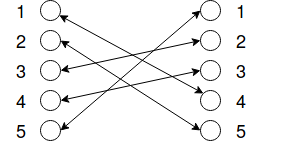
\includegraphics[scale=0.5]{premutation.png}
\end{figure}
\end{columns}
\end{frame}

\begin{frame}{Обратная перестановка}
Для любой перестановки $\varphi \in S_n$ сущесвует обратная перестановка $\varphi^{-1} \in S_n$, такая что 
$\varphi \circ \varphi^{-1} = \varphi^{-1} \circ \varphi  = e$. Она будет иметь вид 

\begin{equation} 
\varphi^{-1} = \left (
  \begin{tabular}{cccc}
  $\varphi$ (1) & $\varphi$ (2) & \ldots & $\varphi$ (n) \\
  1 		 & 2 		  & \ldots & n
  \end{tabular}
\right )
\end{equation}
\end{frame}


\begin{frame}{Понятие назначения}
Мы можем
представлять назначение как некое биективное отображение $\varphi$, которое ставит
элементы конечного множества $\mathrm{U}$ в соотвествие элементам конечного
множества $\mathrm{V}$.
\end{frame}



\begin{frame}{Связь перестановок и назначение}
назначение является перестановкой, которая записывается
в виде

\[
\left (
  \begin{tabular}{cccc}
  1 & 2 & \ldots & n\\
  $\varphi (1)$ & $\varphi (2)$ & \ldots & $\varphi (n)$
  \end{tabular}
\right )
\]
\end{frame}



\begin{frame}{Матрица назначений}
Каждой перестановке множества $\{1, 2, \ldots , n \}$ соответсвует единственная матрица
перестановок $\mathrm{X}_\varphi \in \mathrm{Matrix}_{n \times n}$, элементы котороый определяются как
\[
x_{ij} =
 \begin{cases}
   1 & \text{если } j = \varphi(i) \\
   0 & \text{иначе}
 \end{cases}
\]
Матрицу Х будем называть матрицей назначений
\end{frame}

\begin{frame}{Естественное обобщение ЗОН}
Рассмотрим обобщение ЗОН -- трехиндексную аксиальную задачу о назначениях

Она может быть определена следующим образом. 
Пусть даны $n^3$ весовых коэфициентов $c_{ijk}, (i,j,k=1 \ldots n)$. 
Необходимо найти такие перестановки $\varphi$ и $\xi$, что 
\[
  \min_{\varphi, \xi \in S_n} \sum^n_{i = 1} c_{i \varphi (i) \xi(i)}
\]

где $S_n$ множество всех перестановок целых чисел от $1 \ldots n$.
\end{frame}

\begin{frame}{3-АЗОН как ЗЛП}
Так же задача может быть переписана как задача целочисленного линейного программирования. 

\begin{eqnarray*}
  & \min \displaystyle \sum^n_{i = 1} \displaystyle \sum^n_{j = 1} \displaystyle \sum^n_{k = 1}
  c_{ijk} x_{ijk} \\
  \text{ограничения}
  &\displaystyle \sum^n_{i = 1} \displaystyle \sum^n_{k = 1} x_{ijk} = 1  &(j = 1, \ldots, n) \\
  &\displaystyle \sum^n_{j = 1} \displaystyle \sum^n_{k = 1} x_{ijk} = 1  &(i = 1, \ldots, n) \\
  &\displaystyle \sum^n_{i = 1} \displaystyle \sum^n_{j = 1} x_{ijk} = 1  &(k = 1, \ldots, n) \\
  & x_{ijk} \in \{ 0, 1 \} &(i,j,k = 1, \ldots, n)
\end{eqnarray*}
\end{frame}

\begin{frame}{Известные  алгоритмы}
\begin{itemize}
\item Точный метод ветвей и границ, упорядочивающий полный перебор
\item Алогритмы, выделяющие классы решений из $n-$ мерного многогранника всех возможных решений
\item Подходы для получения оценок точного решения
\item Различные приближенные алгоритмы
\end{itemize}

\end{frame}

\begin{frame}{Алгоритм, сводящий 3-АЗОН к двухмерному виду}
Пусть $\phi = X \rightarrow \mathbb{N}$ -- любая целочислено значащая функция, при этом $1 < \phi_n < n$ 
\begin{enumerate}
\item Берем произвольную подстановку $\pi \in S_n$. Пусть $(d_{jk})$ - $n \times n$ 
матрица, содержащая элементы исходной матрицы $(c_{ijk})$, где индекс $j=\pi(i)$ такой, что
$
d_{ij} = c_{\pi^{-1}(j)jk}
$
для любых $1 \leq j$,$n \leq n$
Положим $f = 0 ; j =1 ; \mathrm{K}={1,2, \ldots , \phi_n}$. 
\item Выберем номер $\sigma(j)$ минимального элемента из множества $\mathrm{argmin} \, \{d_{jk} | k \in K \}$.
\item Полагаем $f = f + d_{j \sigma (j)} ; \mathrm{K} = \mathrm{K}  \setminus  {\sigma(j)} ; k=j+\phi_n$
\item Если $k \leq n $, то $K = K \bigcap {k}$.
\item $j = j + 1$
\item Повторяем п.2, пока j<n. В противном случае идем к п.7
\item Результатом работы алгоритма $\mathrm{A}(\phi_n)$ является значение функции $f$ целевой функции   
$f_{\mathrm{A}(\phi_n)}$. 
\end{enumerate}
\end{frame}

\begin{frame}{Теоретическое обоснование}
Пусть весовые коэфициенты $c_{ijk} \in C$ лежат в отрезке $[a_n, b_n]$, $a_n>0$, $M_n$ -- множество всех возможных $C$. Тогда
\begin{block}{Теорема}
При $b_n / a_n = o(n/ \mathrm{ln} n)$ алгоритм является ассимптотически оптимальным для 3-АЗН на классе матриц $M_n$
и его временная сложность  $O(n^2)$.
\end{block}
\begin{block}{Теорема}
При $b_n / a_n = o(\mathrm{ln} n)$ алгоритм является ассимптотически оптимальным для 3-АЗН на классе матриц $M_n$
и его временная сложность  $O(n \mathrm{ln} n)$. 
\end{block}
\end{frame}

\begin{frame}{Выявленные недостатки. Предлагаемые модификации}
\begin{itemize}
\item Алгоритм чувствителен к выбору начальной перестановки
\item Показна сходимость алгоритма при $n \rightarrow \infty$, что неприменимо в практических задачах
\item Для матрицы, полученной после уменьшения размерности, предлагается использовать 
алгоритм, не гарантирующий лучшее решение.
\end{itemize}

Для исправления этих недостатков предлагаются следующие модификации к алгоритму
\end{frame}

\begin{frame}{Наивный итеративный алгоритм}
\begin{enumerate}
\item Создадим счетчик $q$, изменяющийся от $1$ до $P$
\item $f_{\text{окончательное}} = M$ 
\item \label{naive_p3} Запустим исходный алгоритм, получим $f$ 
\item $f_{\text{окончательное}} = \min \{ f, \text{окончательное} \}$
\item $q = q + 1$, если $q < p$, то идем на шаг \ref{naive_p3}
\item Получено решение  $f_{\text{окончательное}}$
\end{enumerate}
\end{frame}

\begin{frame}{Улучшенный итеративный алгоритм} 
\begin{enumerate}
\item Создадим счетчик $q$, изменяющийся от $1$ до $P$
\item $f_{\text{окончательное}} = M$, $\pi$ -- случайная перестановка
\item \label{smart_p3} Запустим исходный алгоритм с перестановкой $\pi$, получим $f$ 
\item Если $f_{\text{окончательное}} < f$, то
\begin{enumerate}
\item $f_{\text{окончательное}} = f$
\item $g \neq h$ -- два случайных числа, $\pi[g], \pi[h] = \pi[h], \pi[g]$
иначе $\pi$ -- случайная перестановка 
\end{enumerate}
\item $q = q + 1$, если $q < p$, то идем на шаг \ref{smart_p3}
\item получено решение  $f_{\text{окончательное}}$
\end{enumerate}
\end{frame}


\begin{frame}{Модификация с использованием алгоритма поиска точного решения классичесой ЗОН}
\begin{enumerate}
\item Берем произвольную подстановку $\pi \in S_n$. Пусть $(d_{jk})$ - $n \times n$ 
матрица, содержащая элементы исходной матрицы $(c_{ijk})$, где индекс $j=\pi(i)$ такой, что
$
d_{ij} = c_{\pi^{-1}(j)jk}
$
для любых $1 \leq j$,$n \leq n$ \\
Положим $f = 0$
\item Запустим Венгерский алгоритм на матрице $d$ 
\item Результатом работы алгоритма $\mathrm{A}(\phi_n)$ является значение функции $f$ целевой функции   
$f_{\mathrm{A}(\phi_n)}$. 
\end{enumerate}
\end{frame}

\begin{frame}{Модификация целочисленной функции $\phi_n$}
Утверждается, что для любой целочисленной $\phi_n$ алгоритм сходится.
Сложность алгоритма зависит от $\phi_n$ и равна $o(n \phi_n(n) )$
\end{frame}

\begin{frame}{Обзор программного комплекса}
Эксперимент выполнен на языке python3.6

\begin{enumerate}
\item Модуль Premutation
\item Модуль Test
\item Модуль Algorithm
\item Модуль ReportAggregation
\end{enumerate}
\end{frame}

\begin{frame}{Численный эксперимент}
Входные данные эксперимента: 
\begin{itemize}
\item Матрицы различной размерности
\item Матрицы, заполненные по различным правилам
\end{itemize}
\end{frame}

\begin{frame}{Виды матриц}
Матрицы вида $C_{rand}$, сгенерированные случайным образом из~$\{ 1 \ldots n \}$

Матрицы вида $C_{rand}$, которые представляют собой матрицу $c \in C_{rand}$, 
для которой выполнено $c_{ijk} = 0,\quad i,j,k = 1, \ldots, n$

\end{frame}

\begin{frame}{Виды матриц}

Матрицы специального вида $C_{id}$, строящиеся по следующему правилу:
\begin{equation}
c_{ijk} = 
\begin{cases} 
	0, 		&\mbox{i = j = k}  \\
	1,		&\mbox{иначе, }
\end{cases},\quad i,j,k= 1, \ldots, n 
\end{equation}
\end{frame}

\begin{frame}{О методе оценивания}
Предлагается оценивать результат алгоритма и его сходимость через нормализованный вывод 
\begin{equation}
f_{normalized} = \frac{f}{n},
\end{equation} где $f$ -- вывод алгоритма $f$ на матрице размерности $n$.

Ожидается, что для выводов $f^{(n_1)}$, $f^{(n_2)}$ и $f^{(n_3)}$, где $n_3 >> n_2 >> n_1$ значение $\Delta f_{3-2} = f^{(n_3)} - f^{(n_2)}$ будет меньше, чем $\Delta  f_{2-1} = f^{(n_2)} - f^{(n_1)}$:
\begin{equation}
\Delta f_{3-2} < \Delta f_{2-1}
\end{equation}
\end{frame}

\begin{frame}{Результаты рассчета}
\begin{itemize}
\item Алгоритм 2.1  -- исходный алгоритм
\item Алгоритм 2.2 -- наивный итеративный алгоритм
\item Алгоритм 2.3 -- улучшенный итеративный алгоритм
\item Алгоритм 2.4 -- алгоритм с использованием венгерского метода
\end{itemize}

\resizebox{\textwidth}{!}{%
\begin{tabular}{|c|c|c|c|c|c|c|c|c|c|c|}
\hline алгоритм|$n$ & $10$ & $20$ & $50$ & $100$ & $150$ & $500$ & $1000$ & $1250$ & $1500$ & $1750$ \\
\hline Алгоритм 2.1 & $14.61$ & $35.48$ & $103.92$ & $220.28$ & $334.79$ & $1126.03$ & $2253.39$ & $2818.79$ & $3376.94$ & $3946.76$ \\
\hline Алгоритм 2.2 & $14.66$ & $31.32$ & $91.66$ & $194.95$ & $299.87$ & $1043.2$ & $2125.39$ & $2665.64$  & --  & -- \\
\hline Алгоритм 2.3 & $14.42$ & $33.51$ & $94.58$ & $198.18$ & $511.22$ & $1047.52$ & -- & --  & -- &  -- \\
\hline Алгоритм 2.4 & $21$ & $22$ & $50$ & $100$ & $150$ & $501$ &  -- &  -- &  -- & -- \\
\hline
\end{tabular}}
\end{frame}

\begin{frame}{Вывод программы для основного алгоритма со случайно сгенерированными матрицами}

\begin{tabular}{|c|c|c|c|}
\hline $n$ & $f$ & $f_{normalized}$  & $\Delta f_{normalized}$\\
\hline 10 & 14.61 & 1.4610 & -- \\
\hline 20 & 35.48 & 1.7740 & 0.3130 \\
\hline 50 & 103.92 & 2.0780 & 0.3039 \\
\hline 100 & 220.28 & 2.2020 & 0.1240 \\
\hline 150 & 334.79 & 2.2320 & 0.0300 \\
\hline 500 & 1126.03 & 2.2520 & 0.0199 \\
\hline 1000 & 2253.39 & 2.2530 & 0.0010 \\
\hline 1250 & 2818.79 & 2.2550 & 0.0019 \\
\hline 1500 & 3376.94 &  2.2552 & 0.0001 \\
\hline 1750 & 3946.76 & 2.2552 & 0.0 \\
\hline
\end{tabular}
\end{frame}

\begin{frame}{Вывод программы для наивного итеративного алгоритма со случайно сгенерированными матрицами}

\begin{tabular}{|c|c|c|c|}
\hline $n$ & $f$ & $f_{normalized}$ & $\Delta f_{normalized}$ \\
\hline 10 & 14.66 & 1.4660 & -- \\
\hline 20 & 31.32 & 1.5660 & 0.1000 \\
\hline 50 & 91.66 & 1.8332 & 0.2672 \\
\hline 100 & 194.95 & 1.9495 & 0.1163 \\
\hline 150 & 299.87 & 1.9991 & 0.0496 \\
\hline 500 & 1043.2 & 2.0864 & 0.0873 \\
\hline 1000 & 2125.39 & 2.1254 & 0.0390 \\
\hline 1250 & 2665.64 & 2.1325 & 0.0071 \\
\hline
\end{tabular}
\end{frame}

\begin{frame}{Вывод программы для улучшенного итеративного алгоритма со случайно сгенерированными матрицами}
\begin{tabular}{|c|c|c|c|}
\hline $n$ & $f$ & $f_{normalized}$ & $\Delta f_{normalized}$ \\
\hline 10 & 14.42 & 1.442 & -- \\
\hline 20 & 33.51 & 1.6755 & 0.2330 \\
\hline 50 & 94.58 & 1.8916 & 0.2161 \\
\hline 100 & 198.18 & 1.9818 & 0.0902 \\
\hline 250 & 511.22 & 2.0448 & 0.06308 \\
\hline 500 & 1047.52 & 2.0950 & 0.05024 \\
\hline
\end{tabular}
\end{frame}

\begin{frame}{Результат для матриц из $C_{rand}$}
\begin{figure}
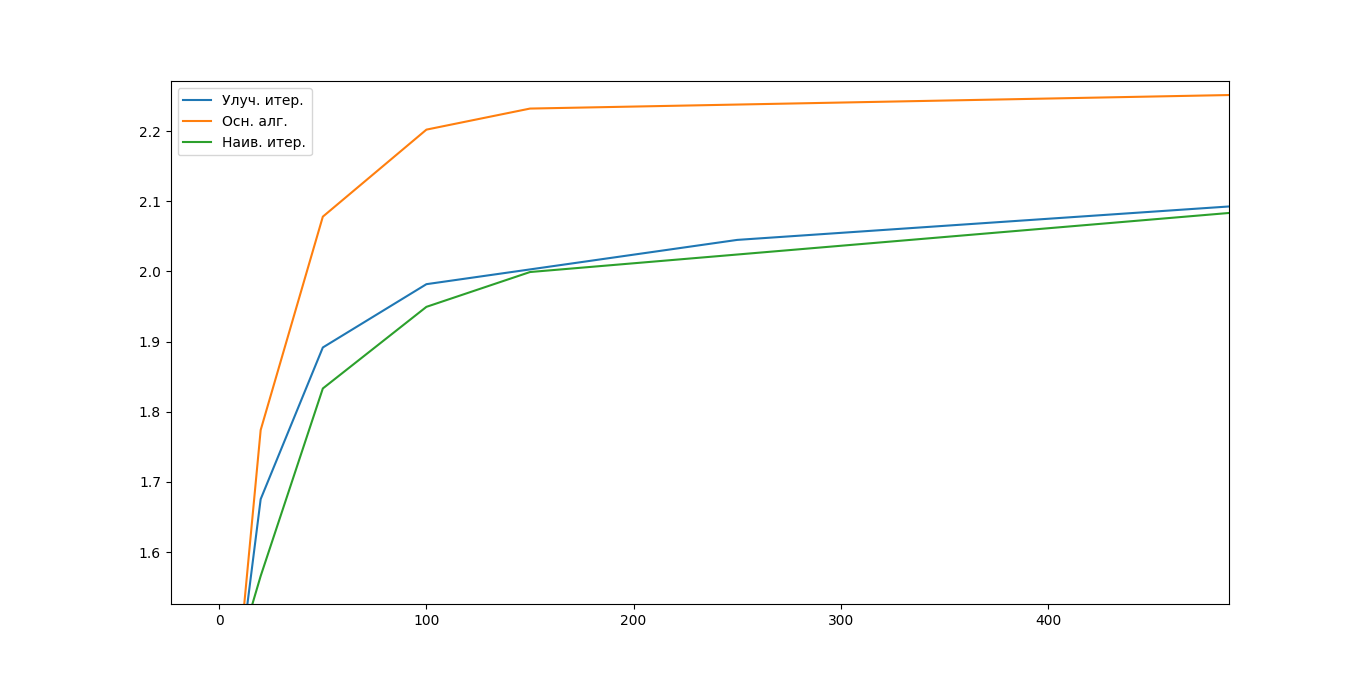
\includegraphics[width=\textwidth]{random_compare.png}
\end{figure}
\end{frame}

\begin{frame}{Вывод программы для основного алгоритма со случайно сгенерированными матрицами с нулевой диагональю}
\label{aglo_rid}
\begin{tabular}{|c|c|c|c|}
\hline $n$ & $f$ & $f_{normalized}$  & $\Delta f_{normalized}$\\
\hline 10 & 14.08 & 1.4080 & -- \\
\hline 20 & 35.84 & 1.7920 & 0.3840 \\
\hline 50 & 103.48 & 2.0696 & 0.2776 \\
\hline 100 & 216.12 & 2.1612 & 0.0916 \\
\hline 250 & 552.48 & 2.20992 & 0.0487 \\
\hline 500 & 1133.76 & 2.26052 & 0.0506 \\
\hline 750 & 1697.91 & 2.26388 & 0.0034 \\
\hline 1000 & 2261.52 & 2.26152 & -0.0024 \\
\hline
\end{tabular}
\end{frame}

\begin{frame}{Вывод программы для наивного итеративного алгоритма со случайно сгенерированными матрицами c нулевой диагональю}
\begin{tabular}{|c|c|c|c|}
\hline $n$ & $f$ & $f_{normalized}$ & $\Delta f_{normalized}$ \\
\hline 10 & 15.08 & 1.5080 & -- \\
\hline 20 & 31.84 & 1.5920 & 0.0840 \\
\hline 50 & 91.96 & 1.8392 & 0.2472 \\
\hline 100 & 195.8 & 1.9580 & 0.1188 \\
\hline 250 & 510.08 & 2.0403 & 0.0823 \\
\hline
\end{tabular}
\end{frame}

\begin{frame}{Вывод программы для улучшенного итеративного алгоритма со случайно сгенерированными матрицами c нулевой диагональю}
\begin{tabular}{|c|c|c|c|}
\hline $n$ & $f$ & $f_{normalized}$ & $\Delta f_{normalized}$ \\
\hline 10 & 13.80 & 1.3800 & -- \\
\hline 20 & 33.32 & 1.6660 & 0.2860 \\
\hline 50 & 92.24 & 1.8448 & 0.1788 \\
\hline 100 & 196.12 & 1.9612 & 0.1164 \\
\hline 250 & 510.56 & 2.0422 & 0.0810 \\	
\hline
\end{tabular}
\end{frame}

\begin{frame}{Результат для матриц из $C_{rid}$}
\begin{figure}
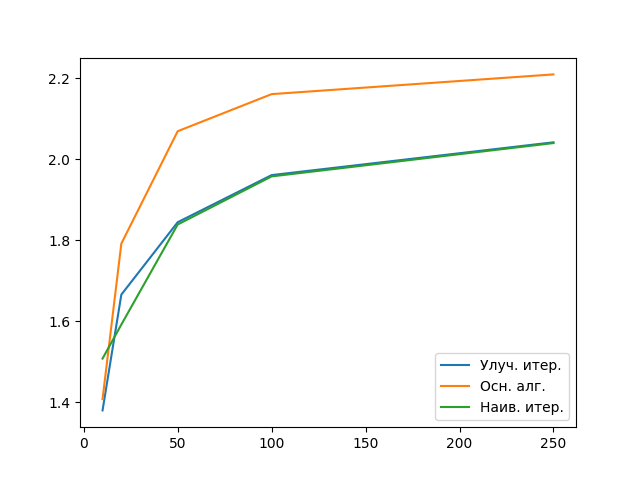
\includegraphics[scale=0.5]{randz.png}
\end{figure}
\end{frame}

\begin{frame}{Результат наивного итеративного алгоритма с матрицами из $C_{rid}$ c различными $\phi_n$}
\begin{eqnarray}
& \phi_n(i) = i \\
 & \phi_n(i) = i \bmod 3
\end{eqnarray}
\begin{figure}
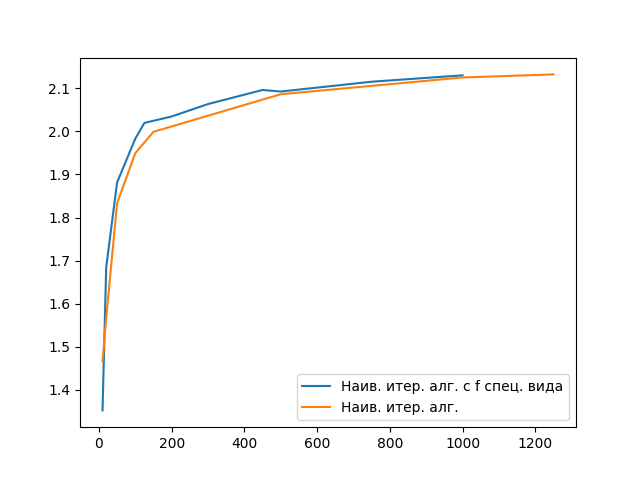
\includegraphics[scale=0.34]{f_vs_nonf.png}
\end{figure}
\end{frame}

\begin{frame}{Вывод программы для алгоритма с использованием венгерского м., $c \in C_{rand}$}
\begin{tabular}{|c|c|c|c|}
\hline $n$ & $f$ & $f_{normalized}$ & $\Delta f_{normalized}$ \\
\hline 10   &  21  & 2.1 & --    \\
\hline 20   &  22  & 1.1 & 1.000 \\
\hline 50   &  50  & 1.0 & 0.000 \\
\hline 100  &  100 & 1.0 & 0.000 \\
\hline 250  &  250 & 1.0 & 0.000 \\ 
\hline
\end{tabular}
\end{frame}

\begin{frame}{Вывод программы для алгоритма с использованием венгерского м., $c \in C_{rid}$}
\begin{tabular}{|c|c|c|c|}
\hline $n$ & $f$ & $f_{normalized}$ & $\Delta f_{normalized}$ \\
\hline 10   & 16  & 1.6   & --  		\\
\hline 20   & 23  & 1.15  & -0.4500 	\\
\hline 50   & 48  & 0.96  & -0.1900 	\\
\hline 100  & 98  & 0.98  & 0.0200 		\\
\hline 250  & 248 & 0.992 & 0.0120 		\\
\hline
\end{tabular}
\end{frame}

\begin{frame}{Вывод программы для алгоритма с использованием венгерского м., $c \in C_{id}$}
\begin{tabular}{|c|c|c|c|}
\hline $n$ & $f$ & $f_{normalized}$ & $\Delta f_{normalized}$ \\
\hline 10   & 16      & 1.6  & -- \\ 
\hline 20   & 23  & 1.15 & -0.4500 \\ 
\hline 50   & 48  & 0.96 & -0.1899 \\ 
\hline 100  & 98   & 0.98 & 0.0200 \\ 
\hline 250  & 248  & 0.99 & 0.0120 \\ 
\hline
\end{tabular}
\end{frame}



\begin{frame}{Вывод}
\begin{cenumerate*}
\item исходный алгорим 2.1 асимптотически сходится, теория подтверждена;
\item предложенные модификации (Алгоритмы 2.2, 2.3, 2.4) асимптотически сходятся, причем сходятся быстрее исходного алгоритма;
\item лучший результат показал алгоритм 2.4 с использованием Венгерского метода. 
\end{cenumerate*}
\end{frame}

\begin{frame}
\begin{cenumerate}
\item Наивная итеративная модификация (алгоритм 2.2) показала себя хорошо.
\item Улучшенная итеративная модификация также показала себя лучше исходного алгоритма, однако, не превосходит
наивную итеративную модификацию
\item Модификация с использованием Венгерского м., показал лучший результат, но он потребляет много памяти
\end{cenumerate}
\end{frame}

\begin{frame}
Спасибо за внимание
\end{frame}
\end{document}
